\documentclass[a4paper, 12pt]{article}
\usepackage{amsfonts,amsmath,amsthm}
\usepackage{graphicx}
\usepackage{authblk}
\usepackage{hyperref}
\usepackage{microtype}
\usepackage{lipsum}
\usepackage[section]{placeins}
% \usepackage{pdflscape}
\usepackage{afterpage}
\usepackage{capt-of}% or use the larger `caption` package
\usepackage{pifont}% http://ctan.org/pkg/pifont
\usepackage{bm}
\usepackage{pdfpages}
\usepackage{mdframed}
\usepackage{makecell}
\usepackage{hyperref}
\usepackage{todonotes}
\usepackage{xcolor}

\DeclareMathOperator*{\argmax}{arg\,max}
\DeclareMathOperator*{\argmin}{arg\,min}
\newcommand{\cmark}{\ding{51}}%
\newcommand{\xmark}{\ding{55}}%

\newtheorem{thm}{Theorem}
\newtheorem{lem}[thm]{Lemma}
\newtheorem{prp}[thm]{Proposition}
\newtheorem{rem}[thm]{Remarks}
\newtheorem{cor}[thm]{Corollary}
\newtheorem{dfn}[thm]{Definition}
\newtheorem{prt}[thm]{Property}
\newtheorem{algo}{Algorithm}

%\def\Dd{$\Delta^d$}
\def\vol{\mbox{vol}}
\def\NN{{\mathbb N}}
\def\RR{{\mathbb R}}
\def \d{{\mathrm d}}
\def \e{{\mathrm e}}
\def \c++{{\tt C++}}
\def\volesti{{\tt volesti}}
\def\cran{{\tt CRAN}}
\def\R{{\tt R}}

\usepackage{geometry}
\geometry{margin=0.7in}

%\usepackage{biblatex}
%\addbibresource{biblio.bib}

\begin{document}
\begin{center}
    \Large{Building a computational toolbox for the analysis of metabolic networks}
\end{center}

%\title{High dimensional uniform sampling and metabolic constrained models}
%\author[1]{Apostolos Chalkis, PhD student in Computer Science}%, \\
%National \& Kapodistrian University of Athens, Greece}
%\maketitle
%\todo[inline]{Avoid passive voice!!! Everywhere. Rewrite if necessary. 
%Avoid "very something". Find the synonym in thesaurus}
%\todo[inline]{Say why the internship will be important for tweag and to the world in general. 
%You will provide them  with something that nobody else has it, but wish to have. Thus there is a demand. 
%For you and volesti, it is rather obvious that it is a nice opportunity.
%I might have to see the call for this.}


\section{Introduction}
%\textcolor{blue}{ \href{http://www.latex-tutorial.com}{LaTeX-Tutorial}}s

Systems biology is an approach in biological and biomedical research. It aims in deciphering the overview and the underlying mechanisms of the phenomena under study. By dictating all the biological levels of organization of living entities, the study of metabolism has been the Holy Grail for Biologists. It is only a few decades that metabolic network reconstruction has allowed for an in-depth insight into the molecular mechanisms of a particular organism by providing models that correlate the genome with molecular physiology. Validation and analysis of such reconstructions allow the identification of key features of metabolism, fundamental for a great range of fields; from the study of ecosystems resilience and restoration to this of inherited and neuro-degenerative diseases and advanced precision medicine. 

The analysis of such metabolic networks however, is in fact a challenging computational problem from the perspective of linear constraint based modelling. Metabolic modelling most commonly used methods, such as \textcolor{blue}{\href{https://www.nature.com/articles/nbt.1614}{Flux Balance Analysis (FBA)}}, is a typical example of a constraint-based metabolic model (CBMM). Thus, the problem of the analysis of a metabolic networks, becomes a computational geometry problem. \textcolor{blue}{\href{https://www.nature.com/articles/s41540-019-0109-0}{Flux Variance Analysis (FVA)}}, \textcolor{blue}{\href{https://dl.acm.org/doi/fullHtml/10.1145/3194656}{computing the polytope's volume}}, 
\textcolor{blue}{\href{https://journals.plos.org/plosone/article?id=10.1371/journal.pone.0235393}{sampling under various distributions from the metabolic network's steady states}} (uniform sampling being of \textcolor{blue}{\href{https://academic.oup.com/bioinformatics/article/33/11/1741/2964731}{special interest}}) are only a few of the constraint-based problems related with the metabolic network analysis. As these are rather challenging problems from the computational point of view, the development of algorithms and software to this end is of high priority.

So far developed software have certain limitations. With respect to uniform sampling for example, random walks scale up to a few hundreds dimensions.  Metabolic networks though, may scale up to dozens sometimes hundreds of thousands dimensions; especially in case of the Human metabolic network as well as in networks derived from microbial communities as those from the human gut microbiome.

Aim of this internship is to contribute to the \textcolor{blue}{\href{https://github.com/GeomScale/volume_approximation}{{\tt volesti}}} \texttt{C++} library in terms of providing a complete \texttt{Python} library toolbox for metabolic network analysis in a highly efficient and user-friendly way. In terms of orders of magnitude, I intend to move from the analysis of a metabolic network of a few dozens of reactions (core network of \textcolor{blue}{\href{http://bigg.ucsd.edu/models/e_coli_core}{\textit{E. coli}}}) to dozens of thousands that the \textcolor{blue}{\href{http://bigg.ucsd.edu/models/Recon3D}{human metabolic network}} implies. I strongly believe that all these contributions will lead to a publication to a top bioinformatics journal. 
%The quest to scale from a few hundreds to a few thousands dimensions is considered as an unquestionably far-reaching goal for many years in computational geometry and statistics.

%From a single cell to the ecosystem level and from a simple biological process to complex phenomena, systems biology has turned the page in modern research, moving from the traditional reductionist research approaches to a new quality. 

%In terms of mathematics, for every constraint-based model of a metabolic network representing \textit{m} metabolites and \textit{n} reactions and regarding the linear case, there is a set $\Omega$ of the feasible fluxes (\textit{v}), where \textit{v} $\in \mathbb{R}^n$, more specifically: $$ \Omega = \{ v\ |\ Sv=0;  l \le v \le u;\ c^Tv=a\}$$ with \textit{S} being the stoichiometric matrix, \textit{l} and \textit{u} the constraints of the system under study, and \textit{a} an optimal value  of a biologically inspired linear objective \textit{c} $\in \mathbb{R}^{3}$. 

%>>>>>>>>> From Tolis 

%Uniform sampling in high dimensions from regions that are defined by linear constraints (i.e.,~convex polytopes), using geometric random walks, is of special interest in numerous scientific fields and applications (e.g.,\ \textcolor{blue}{\href{https://arxiv.org/pdf/2001.04566v1.pdf}{multivariate integration}}, \textcolor{blue}{\href{https://drops.dagstuhl.de/opus/volltexte/2018/8732/}{FinTech}} and  \textcolor{blue}{\href{https://dl.acm.org/doi/10.1145/1008731.1008733}{optimization}}).


 %The package \volesti\ 
%\todo[inline]{I do not see the purpose of mentioning volesti here} is a \c++\ software with an R interface in \cran\ which provides $4$ geometric random walks for uniform sampling and volume computation. It currently scales in a few hundreds dimensions.

%All the open source implementations of random walks scale up to a few hundreds dimensions. The quest to scale from a few hundreds to a few thousands dimensions is considered as an unquestionably far-reaching goal for many years in computational geometry and statistics. 

%Moreover, deciding if a sampling algorithm, or equivalently a Markov chain, converges to a target distribution has theoretical guarantees in high dimensions that are extremely pessimistic for any practical use; hence we need experimental studies to deduce  guarantees.

%My project marks the path towards these challenges. 
%\todo[inline]{The next sentence does not make sense. What is the subject?}
%Hence, on the one hand consists of efficient \c++\ implementations with interfaces in high level programming languages as \R\ and on the other hand performs extended and complex experiments to study the convergence of all the known random walks for uniform sampling for various cases.

%\todo[inline]{Say here in 2 lines what is the internship about}


%\todo[inline]{What are you going to do for tweag?}

%The first goal of this project is to extend \volesti's functionality for uniform sampling by adding all the known random walks that are not currently implemented in \volesti\ and by improving existing ones. The second goal is to implement $3$ diagnostic tools to check convergence of random walks, sampling from multivariate distributions. Third, I stand out a certain application of Flux Balance Analysis (FBA) in metabolic networks with uniform sampling in computational biology \cite{}(see Section~\ref{sec:motivation}).

 %The aim is the first efficient implementation in the thousands in order to extend the limits of contemporary computational tools in certain applications.

 %The diagnostic tools would allow us to experimentally test and compare the speed of convergence (mixing time) of all the known random walks and derive practical bounds for the number of steps required to converge for each one of them. 

 %The aim is to employ the previous practical study to highlight the new implementations as a better and supplementary computational tool to existing ones. 

%Summarizing, at the end of this project, \volesti\ is going to provide all the possible choices for uniform sampling with upper bounds for mixing time derived by extensive experiments. It will also support with efficient {\tt C++} implementations all the necessary routines for FBA in metabolic networks with uniform sampling.

%\todo[inline]{I do not think that they  will print it. So make the footnotes "clickable" with \href to save space.}

\section{Background}

The \textcolor{blue}{\href{https://opencobra.github.io/}{COnstraints Based Reconstruction and Analysis (\texttt{COBRA}) project}} is commonly for the analysis of metabolic networks. Especially the {\tt MATLAB} toolbox provides several implementations of a comprehensive collection of basic and advanced modelling methods. However, the native {\tt MATLAB} code can make the run-time extremely large especially as we move towards more complete and thus complex networks; i.e. moving from lower dimension networks to higher ones.

The package \textcolor{blue}{\href{https://github.com/GeomScale/volume_approximation}{\texttt{volesti}}} is a generic open source \texttt{C++} library, with \texttt{R} and (limited) \texttt{Python} \textcolor{blue}{\href{https://CRAN.R-project.org/package=volesti}{interfaces}}. 
It provides some of the \textcolor{blue}{\href{https://github.com/GeomScale/volume_approximation/wiki}{fastest implementations}} for high dimensional Monte Carlo sampling and volume approximation able to scale up to a few thousands of dimensions and already tested on copula estimation for financial modelling. It is the main package of the open source organization \textcolor{blue}{\href{https://geomscale.github.io/}{{\tt GeomScale}}}, which has been accepted as a mentoring organization by the \textcolor{blue}{\href{https://summerofcode.withgoogle.com/organizations/5673184117915648/}{Google Summer of Code 2020}}.

The run-time of \texttt{volesti} is \textcolor{blue}{\href{https://github.com/GeomScale/volume_approximation/wiki/volesti-vs-cobra-toolbox}{two order of magnitude smaller than \texttt{COBRA}}} for small metabolic networks and can be even smaller for high dimensional networks as it is equipped with more sophisticated algorithms and implementations. However, the software of \texttt{volesti} has not been designed according to the needs of metabolic network analysis. Thus, it lacks of preprocess routines and general (algorithmic and coding) optimizations to be considered as a benchmark package for high dimensional metabolic network analysis.

%Aim of this internship is to contribute to the \textcolor{blue}{\href{https://github.com/GeomScale/volume_approximation}{{\tt volesti}}} \texttt{C++} library in terms of providing a complete \texttt{Python} library toolbox for metabolic network analysis in a highly efficient and user-friendly way.
%\texttt{volestipy} will include all the current \texttt{volesti} functions, but also those that the GeomScale group is developing now. Furthermore, functions specialized for the analysis of polytopes derived from metabolic network, will be developed and included in this Python interface of \texttt{volesti}. Finally, the need for supporting sampling and rounding such polytopes of high dimensions will be addressed and extended tests will be performed in high dimensional metabolic networks. %In terms of orders of magnitude, I intend to move from the analysis of a polytope of a few dozens of reactions (core network of \textcolor{blue}{\href{http://bigg.ucsd.edu/models/e_coli_core}{\textit{E. coli}}} to dozens of thousands that the \textcolor{blue}{\href{http://bigg.ucsd.edu/models/Recon3D}{human metabolic network}} implies. 


%I will enhance the \texttt{Python} interface of the open source package \texttt{volesti} with sampling methods, diagnostic tools, prepossessing routines and high quality interfaces and visualization tools for sampling-based metabolic flux analysis (SMFA). In terms of orders of magnitude, I intend to move from the analysis of a polytopes of a few dozens of reactions (core network of \textcolor{blue}{\href{http://bigg.ucsd.edu/models/e_coli_core}{\textit{E. coli}}} to dozens of thousands that the \textcolor{blue}{\href{http://bigg.ucsd.edu/models/Recon3D}{human metabolic network}} implies. 


%In its current version, it provides three geometric random walks for sampling (including CDHR and BiW) and two state-of-the-art methods for volume estimation for convex polytopes. \texttt{volesti} supports sampling up to a few hundreds of dimensions. Being a C++ software as well as the sampling algorithms included, make volesti a rather fast option for CBMM studies. 

 %The are also {\tt C++} \textcolor{blue}{\href{https://github.com/rzrsk/vaidya-walk}{implementations}} for Dikin/Vaidya/John walk based on the same {\tt C++} library with \texttt{volesti} for linear algebra operations (i.e.\ {\tt Eigen}).

%\textcolor{blue}{\href{https://www.ncbi.nlm.nih.gov/pubmed/12000313}{SMFA}} can be used to study any biological system that can be modeled by a metabolic network; a \textcolor{blue}{\href{https://www.ncbi.nlm.nih.gov/pmc/articles/PMC6718391/}{powerful tool}} which has not fully exploited due to costly computations. The open source package \textcolor{blue}{\href{https://opencobra.github.io/}{{\tt opencobra}}} provides two algorithms for uniform sampling, combined with several routines for SMFA. Interestingly, the default random walk in {\tt opencobra} (i.e.\ CDHR) performs $\sim 100$ times slower than the corresponding implementation in \texttt{volesti}. 

%metabolic modelling, is among those scientific fields that need such approaches the most to address their modern challenges. Flux Balance Analysis (FBA) is a typical example of a constraint-based metabolic model (CBMM) [2].

%High dimensional uniform sampling from convex polytopes is an active research area in computational geometry and statistics with a wide range of applications.
%An extended introduction to geometric random walks is presented in this \textcolor{blue}{\href{https://www.cc.gatech.edu/~vempala/papers/survey.pdf}{survey}}, while 

%The $3$ diagnostic tools combined with the new rounding methods will allow us to experimentally test and compare the speed of convergence (mixing time) of all the known random walks and derive practical bounds for the number of steps required to converge for each one of them. I will employ the previous practical study to highlight the new implementations as a better and supplementary computational tool to existing ones (e.g.,\ {\tt opencobra}) for SMFA. Last but not least, I plan the practical study on mixing time to lead to a paper submission to an international conference on statistics.

%The best theoretical results for the mixing times are precisely displayed in \textcolor{blue}{\href{https://arxiv.org/abs/1911.05656}{Table~1, p.~3}}. There are two random walks, i.e.,\ Coordinate Hit and Run (CDHR) and Billiard walk, for which there are not theoretical mixing times but they are both implemented in \volesti.

%Table 1 shows the implementations of this project. After $12$ weeks I will have extended \volesti's functionality with the implementations of all the known random walks for uniform sampling and I will improve the existing one. 

\section{Motivation}\label{sec:motivation}
Main outcome of this project will be a benchmark \texttt{Python} library, namely \texttt{volestipy}, for a series of constraint-based problems, for the needs of the metabolic networks analysis. This will allow for 
%a \textit{one-stop-shop} \texttt{Python} library for 
the analysis of high dimensional real data metabolic networks analysis. More specifically, it will allow the implementation of the complete analysis of networks, in some cases for the first time to my knowledge, and it will provide a fundamental first step for the analysis of networks of networks, for the case of microbial communities as the ones in human gut, a highly important field for biomedical research.
The biomedical community will have a great benefit from powerful implementations of optimization methods, high dimensional Monte Carlo sampling, and preprocess methods for the study of \textcolor{blue}{\href{https://www.frontiersin.org/articles/10.3389/fcimb.2020.00052/full}{infectious diseases}}, \textcolor{blue}{\href{https://www.sciencedirect.com/science/article/pii/S155041311730092X}{precision medicine}}, \textcolor{blue}{\href{https://www.sciencedirect.com/science/article/pii/S1359644613002481}{drug discovery}} and more. 

%Faster and of high quality sampling methods, capable of dealing with high dimensional networks would benefit the most the metabolic modelling at the genome-scale. 
%Implementations of Coordinate Directions Hit-and-Run (CDHR) and Billiard walk (BiW) can provide fast and high quality sampling, however they are not included in \texttt{cobrapy} (the Python interface of COBRA). 

%This project will significantly update \texttt{volesti} to the first package that contains efficient implementations of all the existing random walks for uniform sampling, scaling up to thousands dimensions. 

%Having knowledge --\textcolor{blue}{\href{https://www.slideshare.net/ApostolosChalkis/14th-athens-colloquium-on-algorithms-and-complexity-acac19}{from my existing research work}}-- of the fact that the actual mixing time of certain random walks is better than that given in theory, I expect this experimental study to lead to innovative results useful to research and business communities which wish to employ such computational tools and perform Monte Carlo simulations. The project will also provide efficient {\tt C++} implementations for all the necessary routines of SMFA, extending the limits of contemporary computational tools. The latter will be a road-map to test constraint-based metabolic modelling with uniform sampling at the ecosystem level (e.g.\ using the data from \textcolor{blue}{\href{https://www.biorxiv.org/content/10.1101/857391v1}{here}}) for the first time. I also intent to further work on SMFA employing the computational tools of this project and providing a new algorithmic and mathematical framework to study metabolic networks. I strongly believe that this project and its potentials will greatly benefit organizations like {\tt Tweag} which are interested in Bayesian inference, Markov Chain Monte Carlo methods and bioinformatics. I hope it will serve as a building block towards a long lasting cooperation for the development of the best open source randomized algorithms and computational tools based on sampling from multivariate distributions and efficient implementations.

%I hope that this project will also be a road-map towards efficient open source implementations related to sampling and randomized algorithms  for multivariate sampling for more general families of distributions (e.g.\ log-concave densities) and randomized algorithms for convex optimization. %(for more details and references for all the above see the Appendix).% Moreover, it will be beneficial to educational communities and university students as it would help them to build intuition as well as it can serve as a platform for student projects.

%Thus this project is expected to be beneficial to both (a) educational and (b) research open source communities. For (a) university students studying computational geometry, statistics or convex analysis will have access to an efficient library that will help them build intuition as well as it can serve as a platform for student projects. 
%About (b) researchers could use the library in their research projects and also extend it according to their needs.

\section{Project Description}
\texttt{volestipy} will include all the current \texttt{volesti} functions, but also new implementations of optimization methods needed for FBA and FVA, new Monte Carlo sampling algorithms and new preprocessing and coding optimizations.
The main part of the implementation will be given in \texttt{C++} but also in \texttt{Python} and \texttt{Cython} as a natural extension of the current version of the \texttt{volesti} library and its wrapping in \texttt{Python} correspondingly. 
The code will be merged into the \texttt{volesti} software and will lead to an updated version of the package. %In Table~\ref{tab:impmeth} modifications, additions on the existing code and implementations of the \texttt{volestiPy} library proposed are shown.

%\begin{figure}[!h]
%  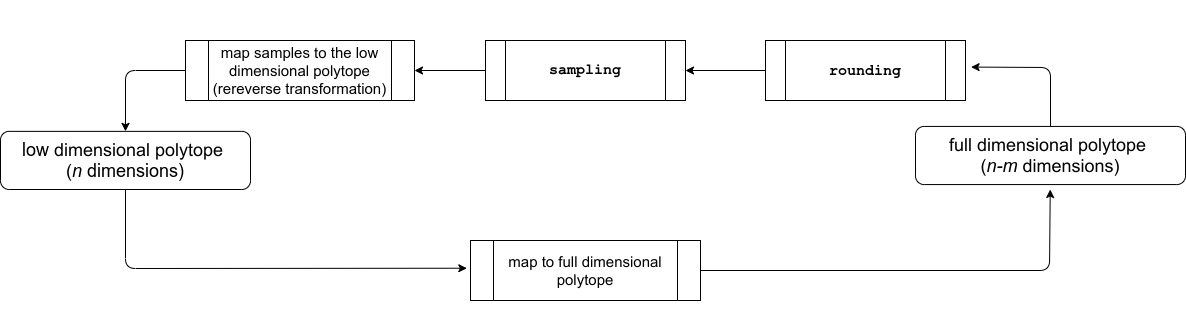
\includegraphics[width=\linewidth]{sampling_pipeline.png}
%  \caption{Steps for sampling a polytope derived from a metabolic network.}
%  \label{fig:Pipeline}
%\end{figure}

The project will be considered as successful if (a) the implementations of the timeline Table will result to a new \texttt{Python} package, namely \texttt{volestipy}, and (b) \texttt{volestipy} can perform a complete analysis for the latest human metabolic network. %The practical study of random walks will also lead to a submission to an international conference of computational statistics.

%\begin{flushleft}
%\begin{table}[h!]
%\footnotesize
%\centering
%\begin{tabular}{|l|c|}
%\hline
%\hspace{1.6cm} Implementation & Type \\ \hline% & References \\ \hline\hline
%1. PSRF / RL / GEW & Diagnostic tools \\ \hline%& \cite{Hewson15} / \cite{Raftery92} / \cite[p.~8]{Kathryn96} \\ \hline
%2. Improved Billiard walk & random walk \\ \hline%& \cite{Polyak14} \\ \hline
%3. Dikin / Vaidya / John walk & random walks \\ \hline% &  \cite{Vaidyawalk} \\ \hline
%4. Two polytope rounding methods & prepossessing \\ \hline% & \cite{Haraldsdottir17, Cousins15} \\ \hline
%5. \R\ interface for FBA analysis & application \\ \hline% &   \\ \hline
%\end{tabular}
%\caption{\label{tab:impmeth} The proposed implementations during Tweag Fellowship.}
%\end{table}
%\end{flushleft}

\textbf{Mentors}: \textcolor{blue}{\href{https://vissarion.github.io/}{Vissarion Fisikopoulos}}s sofware Engineer \& Research Scientist at University of Athens and Oracle and %, he has long experience in open source software development.\\
\textcolor{blue}{\href{https://who.paris.inria.fr/Elias.Tsigaridas/}{Elias Tsigaridas}}, research scientist at INRIA Paris.% and an expert on algebraic algorithms and mathematical software.

\section{Timeline}

\begin{table}[h!]
%\footnotesize
\centering
\begin{tabular}{|c|c|}\hline
 Week & Description \\ \hline\hline
 1st, 2nd & Develop FBA and FVA functions for the \texttt{volestipy} package \\ \hline
 3rd & \begin{tabular}[c]{@{}c@{}}Implement preprocess methods and code \\ optimizations on existing implementations\end{tabular}\\ \hline
 4th \& 5th & \begin{tabular}[c]{@{}c@{}}Build the \texttt{Python} interface including FBA, FVA, \\ Monte Carlo sampling and preprocess methods\end{tabular} \\ \hline
 6th & Develop visualization modules for each of the \texttt{volestipy} modules \\ \hline
 7th \& 8th & \begin{tabular}[c]{@{}c@{}}Test algorithms' scalability in real data of metabolic \\ networks and make further code optimizations\end{tabular}
 \\ \hline
 9th, 10th \& 11th & \begin{tabular}[c]{@{}c@{}} Perform a complete analysis of high dimensional metabolic \\ networks included the latest \textcolor{blue}{\href{http://bigg.ucsd.edu/models/Recon3D}{human metabolic network}} \end{tabular}  \\ \hline
%9th, 10th \& 11th & \begin{tabular}[c]{@{}c@{}}Fix, improve and develop the \texttt{volestipy} library \\ according to the issues derived on week $8$\end{tabular}  \\ \hline
 12th & \makecell{Write the documentation and useful examples} \\ \hline
\end{tabular}
\end{table}

\end{document}

